\documentclass[a4paper,twocolumn]{article}

\usepackage[utf8]{inputenc}
\usepackage[francais]{babel}
\usepackage{graphicx}
\usepackage{caption}
\usepackage[left=2cm, right=2cm, top=2cm, bottom=2cm]{geometry}
\usepackage{amsmath}

\title{Détection de cercles avec la transformée de Hough}

\author{
	Sébastien Klasa - Polytech Paris-Sud\\
	\texttt{klasa.sebastien@gmail.com}
}

\date{3 janvier 2019}

\begin{document}

\maketitle

\section{Exercice 1}

\paragraph{Question 1} Pour $\delta r = 2$ nous aurons $\left\lfloor \frac{r_{max} - r_{min}}{\delta r} \right\rfloor = 49$ valeurs discrètes. Pour $\delta r = 0.5$ nous aurons $198$ valeurs.

\paragraph{Question 2} Nous pouvons décrire $\left\lfloor \frac{r_{max} - r_{min}}{\delta r} \right\rfloor \times \left\lfloor \frac{c_{max} - c_{min}}{\delta c} \right\rfloor \times \left\lfloor \frac{rad_{max} - rad_{min}}{\delta rad} \right\rfloor = 1332936$ cercles avec ces trois variables.

\paragraph{Question 3} $acc(1,1,1)$ correspond au cercle de rayon 1 centré en $(1,1)$. $acc(10,7,30)$ correspond au cercle de rayon 30 centré en $(10,7)$.

\paragraph{Question 4} La case associée est $acc(40,40,13)$.

\section{Exercice 2}

Avant tout traitement, j'applique un léger filtre gaussien pour atténuer le bruit. Ensuite, j'applique un filtre de Sobel pour détecter les contours. Cette image des contours me permet d'incrémenter l'accumulateur par la magnitude des pixels des cercles.

Pour éviter de privilégier les cercles plus grands, je normalise les valeurs de l'accumulateur par le périmètre du cercle associé. Je cherche ensuite les maxima locaux pour finalement sélectionner les $n$ plus grands.

Les figures \ref{detection_four}, \ref{detection_fourn} et \ref{detection_coins} sont quelques exemples de détection de cercles.

\begin{figure}[h]
	\centering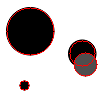
\includegraphics{images/detection_four.png}
	\caption{Exemple de détection de cercle.}
	\label{detection_four}
\end{figure}

\begin{figure}[h]
	\centering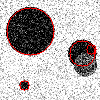
\includegraphics{images/detection_fourn.png}
	\caption{Exemple de détection de cercle.}
	\label{detection_fourn}
\end{figure}

\begin{figure}[h]
	\centering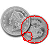
\includegraphics{images/detection_coins.png}
	\caption{Exemple de détection de cercle.}
	\label{detection_coins}
\end{figure}

\section{Exercice 3}

\paragraph{Question 1} Le temps de calcul nécessaire pour l'image four.png est 2150 ms. La complexité en $O(n^4)$ peut être expliquée par le fait que nous parcourons tous les pixels de l'image ($O(n^2)$) pour chaque ligne et chaque colonne de l'accumulateur. Le temsp estimé pour une image de 600 px est $2150 \text{ ms } \times 100^{-4} \times 600^4 = 2786400 \text{ ms } = 46.44 \text{ minutes }$.

\end{document}